\chapter{Least Squares method}\label{LSmethodChapter}

As we have seen in previous chapters the overall process to determine the location of the source is studying the correlation between the VTEC value and the solar-zenith angle (or source-zenith angle, speaking in general terms) for a possible location.

That is, for an IPP with a location and an associated VTEC value, given the location of a possible source, compute the cosine between them, and see that the closer the cosine is to 1 (or 180$^{\circ}$), the higher the VTEC value.

The idea that we wanted to test with this method was finding the location of the source by performing the inverse operation: having the VTEC, location of the IPP and correlation (1, assuming a near-linear correlation), obtaining the source's right ascension and declination.

\section{The system of equations}

The source-zenith cosine between the source and the IPP was computed using the following equations:

\begin{equation} \label{eq:61}
unitVectorIPP =
\begin{bmatrix}
X' \\
Y' \\
Z'
\end{bmatrix}
=
\begin{bmatrix}
\cos\delta_{g} * \cos\alpha_{g} \\
\cos\delta_{g} * \sin\alpha_{g} \\
\sin\delta_{g}
\end{bmatrix}
\end{equation}

\begin{equation} \label{eq:62}
unitVectorSource =
\begin{bmatrix}
X \\
Y \\
Z
\end{bmatrix}
=
\begin{bmatrix}
\cos\delta_{s} * \cos\alpha_{s} \\
\cos\delta_{s} * \sin\alpha_{s} \\
\sin\delta_{s}
\end{bmatrix}
\end{equation}

\begin{equation} \label{eq:63}
\cos \chi = unitVectorIPP \cdot unitVectorSource
\end{equation}\\

Having the VTEC and source-zenith cosine, we could find the correlation of the two variables, expecting that the real source would yield a near-linear correlation.

Visually, we can see the relation between VTEC and the computed cosine in figure \ref{fig:solar-zenith-angle}, obtained in chapter 3 when studying the a specific case for the Sun.

\begin{figure}[!htb]
	\begin{centering}
		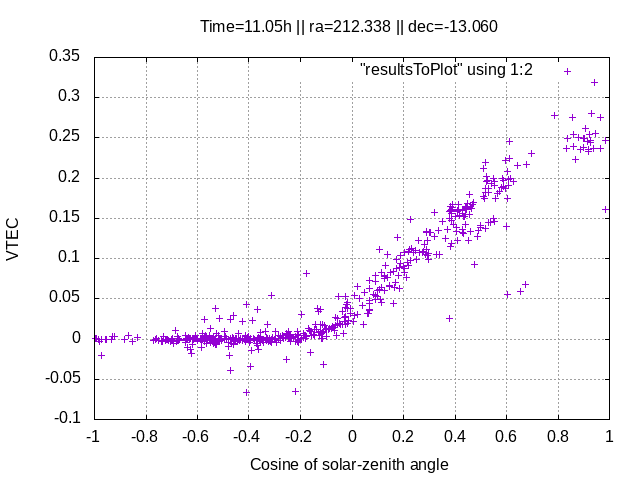
\includegraphics[width=0.5\linewidth]{images/ch4/resultSunTest.png}
		\caption{VTEC as a function of the solar-zenith angle's cosine}
		\label{fig:solar-zenith-angle}
	\end{centering}
\end{figure}

As we have previously seen for this case, there appears to be a linear relation starting around $\cos \chi = -0.1$ between the two studied parameters. Therefore, we could define this linear relation as a \textbf{straight line} ($y = mx + b$) by expressing the estimated VTEC value ($\Delta V$) as a function of the source-zenith cosine (\ref{eq:linearRelation}).

\begin{equation} \label{eq:linearRelation}
\Delta V = a\cos \chi + b
\end{equation}

Because the cosine is computed using the previous equations (\ref{eq:61}, \ref{eq:62}, \ref{eq:63}). It can be expressed as follows, the dot product of both unit vectors:

\begin{equation} \label{eq:cosine}
\cos \chi = XX' + YY' + ZZ'
\end{equation}

Where $X'$, $Y'$, $Z'$ are the components of the IPP's unit vector obtained from equation \ref{eq:61}, and $X$, $Y$, $Z$ are the unknowns of our equation: the components of the source's unit vector, which could be used to easily find the right ascension and declination of the source by using trigonometric operations.

However, finding the value of these unknowns is the challenge of this method. Taking the cosine as \ref{eq:cosine} we can express the linear function as:

\begin{equation} \label{eq:substitute}
\Delta V = aXX' + aYY' + aZZ' + b
\end{equation}

Because $a$ and $b$ are unknowns as well as $X$, $Y$ and $Z$, we can group them as follows:

\begin{equation} \label{eq:newNames}
\Delta V = \alpha X' +  \beta Y' +  \gamma Z' + b
\end{equation}

Our aim after solving the previous equation would be obtaining the values of $X$, $Y$ and $Z$. We can see that:

\begin{equation} \label{eq:elTrucoDelAlmendruco}
\sqrt{\alpha^{2}+\beta^{2}+\gamma^{2}} = \sqrt{a^{2}(X^{2}+Y^{2}+Z^{2})} = \sqrt{a^{2}} = a
\end{equation}

Because $X$, $Y$ and $Z$ are the components of a unit vector\footnote{$\sqrt{(X^{2}+Y^{2}+Z^{2})} = 1$}. The previous allows us to, once we know the values of $\alpha$, $\beta$ and $\gamma$, obtain $X$, $Y$ and $Z$ by doing:

\begin{equation} \label{eq:iso}
\frac{\alpha}{\sqrt{\alpha^{2}+\beta^{2}+\gamma^{2}}} = \frac{\alpha}{a} = \frac{aX}{a} = X
\end{equation} \\

In our data we can find, for each IPP: $\Delta V$, $X'$, $Y'$, $Z'$ (because we have the right ascension and declination of the point).

For each of these IPPs, we have an equation of the form $\Delta V = \alpha X' +  \beta Y' +  \gamma Z' + b$ and, therefore, we have an overdetermined system of equations, with more equations (unknown, depends on the input data) than variables (four: $\alpha$, $\beta$, $\gamma$ and $b$)

Knowing how to obtain $X$, $Y$ and $Z$ from $\alpha$, $\beta$ and $\gamma$, we can now focus on solving the system of equations to obtain the latter unknowns .

Because we have an overdetermined system of equations, the solution can be approximated using the \textbf{Least Squares} approach. 

Least Squares is a method to estimate the solution of an overdetermined system of equations (more equations than unknowns, as in our case), by minimizing the sum of the squared residuals. Residuals will be studied in more detail in the lasts sections of this chapter.

The method estimates the solution of a matrix system of the form $y = AX$ using the following equation:

\begin{equation}\label{eq:mainEq}
X = (A^{T}A)^{-1}A^{T}y
\end{equation} 

Our system can be represented in matrix form  as follows:

\begin{equation} \label{eq:matrixSystem}
\begin{bmatrix}
\Delta V_{0} \\
\Delta V_{1} \\
. \\
. \\
. \\
\Delta V_{n}
\end{bmatrix}
=
\begin{bmatrix}
X'_{0} & Y'_{0} & Z'_{0} & 1 \\
X'_{1} & Y'_{1} & Z'_{1} & 1 \\
. & . & . & .\\
. & . & . & .\\
. & . & . & .\\
X'_{n} & Y'_{n} & Z'_{n} & 1 \\
\end{bmatrix}
\begin{bmatrix}
\alpha \\
\beta \\
\gamma \\
b \\
\end{bmatrix}
\end{equation}

Where y is the VTEC, A the components of the IPP, and X the solution to the system, $\alpha$, $\beta$, $\gamma$ and $b$.

With the Least Squares method we could obtain $X$, $Y$ and $Z$ using the solution to the system ($\alpha$, $\beta$, $\gamma$). Taking into consideration equation \ref{eq:62}, the values of the right ascension and declination angles can be obtained by performing the inverse trigonometrical operations, that is:

Because we know that $Z=\sin(\delta_{s})$ we the declination is obtained by simply computing the arc sinus:

\begin{equation} \label{eq:inverseTrigoTriennal}
\delta_{s} = \arcsin(Z)
\end{equation}

But we have two operations that involve the declination, $X=\cos\delta_{s} * \cos\alpha_{s}$ and $Y=\cos\delta_{s} * \sin\alpha_{s}$. Both involve $\cos\delta_{s}$ so we can equate them:

\begin{equation} \label{eq:rmCos}
\frac{Y}{\sin\alpha_{s}} = \frac{X}{\cos\alpha_{s}}
\end{equation}


\begin{equation} \label{eq:inverseTrigoAtan}
\alpha_{s} = \text{arctan2}(X,Y)
\end{equation}

The $\text{arctan2}(X,Y)$ function is a Fortran function that computes the tangent but using two numbers. Instead of relying only on one angle (which would cause ambiguity regarding the quadrant of the angle) this function uses both angles to determine the exact value, which suits our situation.

Using these two operations, the algorithm finally yields our solution: the right ascension and declination estimated from using all the IPPs' information as an overdetermined system.

Furthermore, another possibility would be executing the algorithm multiple iterations. Using the estimated location yielded by each iteration, the algorithm would compute the cosine of the angle between the estimated solution and the IPP (each line) and discard it considering a certain cosine threshold: -0.1 in particular, the cosine in which the linear relation starts (day hemisphere in the case of the Sun) as we have seen in previous chapters. The results of the algorithm with and without iterations are discussed in the last section.

The main advantage of this method over the one introduced in the previous chapter is that it does not need to compute the correlation (which requires passing the data set once) every time a location is considered. The data set itself (the) file is only traversed once.

\section{Pseudocode}

The following is the pseudocode of the algorithm for a single iteration of the algorithm:

\begin{algorithm}
	\caption{Least Squares method}\label{leastSquaresPseudo}
	\begin{algorithmic}[1]
		\Procedure{main}{}
		
		\For {i each line in file}
		\State $\textit{y(i)} \gets \text{vtec}$
		\State $\textit{A(i,0)} \gets \text{cos(dec)*cos(ra)}$
		\State $\textit{A(i,1)} \gets \text{cos(dec)*sin(ra)}$
		\State $\textit{A(i,2)} \gets \text{sin(dec)}$
		\State $\textit{A(i,3)} \gets \text{1}$
		\EndFor
		
		\State $\textit{sytemSolution} \gets (A^{T}A)^{-1}A^{T}y$
		
		\Return $obtainEstimatedPosition(sytemSolution)$
		\EndProcedure

		\Procedure{$obtainEstimatedPosition(systemSolution)$}{}
			\State $\textit{a} \gets sytemSolution(0)$
			\State $\textit{b} \gets sytemSolution(1)$
			\State $\textit{g} \gets sytemSolution(2)$
			\State $\textit{mod} \gets \sqrt{a^{2} + b^{2} + g^{2}}$ 
			
			
			\State $\textit{X} \gets a/mod$
			\State $\textit{Y} \gets b/mod$
			\State $\textit{Z} \gets g/mod$
			
			\State $\textit{dec} \gets arcsin(Z)$
			\State $\textit{ra} \gets arctan(X,Y)$
			
			\Return $(ra, dec)$
		\EndProcedure
	\end{algorithmic}
\end{algorithm}

The algorithm first stores the necessary data in the arrays and uses them to compute the system solution. The estimated location of the source is then obtained from the system solution by means of the equations presented in the previous section.

\clearpage

\section{Implementation}

For the case of no iterations, the algorithm can simply be implemented by storing each line of information in an array. On the other hand, when discarding outliers using the result of the previous iteration, two possible implementations exist:

\begin{itemize}
	\item Using the same static array for all iterations, but storing 0s in the rows of unused IPP information
	\item Using a dynamical, allocatable array, storing only the information that will be used
\end{itemize}

When using dynamical arrays in Fortran these have to be allocated/deallocated, the following is the function that adds a new row to the array storing the information, implemented for our case with 4 columns and an unknown number of rows.

\begin{minipage}{\linewidth}
\begin{lstlisting}[style=myFortranStyle, caption=Adding a new row to a two dimensional array]
subroutine addRowToArray(array, elem0, elem1, elem2, elem3)
	implicit none
	integer :: i, oldSize
	double precision, intent(in) :: elem0, elem1, elem2, elem3
	double precision, dimension(:,:), allocatable :: array
	double precision, dimension(:,:), allocatable :: tmpArray

	if(allocated(array)) then
		! Allocate one more row to the tmpArray
		oldSize = size(array,1)
		allocate(tmpArray(0:oldSize, 0:3)) 

		! Copy the original content of the array
		tmpArray(0:oldSize,0:3) = array(0:oldSize,0:3)

		! Append the new row
		tmpArray(oldSize,0) = elem0
		tmpArray(oldSize,1) = elem1
		tmpArray(oldSize,2) = elem2
		tmpArray(oldSize,3) = elem3

		! Free the previous array and store the new data in it
		deallocate(array)
		call move_alloc(tmpArray, array)
	else
		allocate(array(0:0, 0:3))
		array(0,0) = elem0
		array(0,1) = elem1
		array(0,2) = elem2
		array(0,3) = elem3
	end if
end subroutine addRowToArray\end{lstlisting}
\end{minipage}

The function first checks if the array is already allocated, in which case the previous array is copied to a new one with one more row and then the new elements are stored in the it with the new space. If it has not been allocated yet, a new array is created but with one single row.

Because of this, each time a new row is added, the processed data up until that point has to be traversed again (when copying the content of the array to the new one).

On the other hand, using a static array allows us to store the data in one single pass (simply storing 0s if we are not going to use the data), consequently, using the approach with dynamic arrays has more time complexity.

Both methods yield exactly the same results, as the rows that contain 0s are not used in the matrix computations, because of this, the algorithm works with the static version, to assure that there is only a single pass of the data.

The following is the main function of the algorithm, which stores the data in the array reading it from the input file (listing \ref{lst:storeData}), computes the solution to the system (listing \ref{lst:solveSystem}), and then using that solution obtains the estimated location of the source (listing \ref{lst:obtainSource}). \\

\begin{minipage}{\linewidth}
	\label{lst:main}
	\begin{lstlisting}[style=myFortranStyle, caption=Main Least Squares function]
	subroutine leastSquares(iteration, solutionRa, solutionDec)
		implicit none
		integer, intent(in) :: iteration
		double precision :: solutionRa, solutionDec
		double precision, dimension(0:numRows) :: matrixVTEC
		double precision, dimension (0:numRows, 0:3) :: matrixIPP
		double precision, dimension (0:3) :: solution
		
		call storeMatrixData(matrixVTEC, matrixIPP, iteration, solutionRa, solutionDec)
		call matrixComputations(solution, matrixIPP, matrixVTEC)
		call obtainSourceLocation(solution, solutionRa, solutionDec)
	
	end subroutine leastSquares\end{lstlisting}
\end{minipage}

The static storeMatrixData function traverses the file and stores the information, if the method is working with multiple iterations, it also checks using the past iteration's estimation whether the IPP point is valid or not. If it is, the components are computed with function computeComponentsIPP() (listing \ref{lst:computeComponents}), otherwise, 0s are stored for that row.

\begin{minipage}{\linewidth}
	\label{lst:storeData}
	\begin{lstlisting}[style=myFortranStyle, caption=Storing the data from the input file]
	subroutine storeMatrixData(matrixVTEC, matrixIPP, iteration, solRa, solDec)
		implicit none
		integer, intent(in) :: iteration
		double precision, intent(in) :: solRa, solDec
		double precision, dimension(0:numRows) :: matrixVTEC
		double precision, dimension (0:numRows, 0:3) :: matrixIPP
		double precision :: vtec, raIPP, decIPP
		double precision :: xIPP, yIPP, zIPP
		integer :: i, validSample
		
		call openFile(inputFileName)
		
		do i = 0, numRows
			read (1, *, end = 240) vtec, raIPP, decIPP
			validSample = 1
			if (iteration /= 0) then
				validSample = checkOutlier(solRa, solDec, raIPP, decIPP)
			end if
			if (validSample == 1) then
				call computeComponentsIPP(raIPP, decIPP, xIPP, yIPP, zIPP)
			else
				vtec = 0
				xIPP = 0
				yIPP = 0
				zIPP = 0
			end if
			matrixVTEC(i) = vtec
			matrixIPP(i, 0) = xIPP
			matrixIPP(i, 1) = yIPP
			matrixIPP(i, 2) = zIPP
			matrixIPP(i, 3) = 1
		end do
		240 continue
		close(1)
	end subroutine storeMatrixData\end{lstlisting}
\end{minipage}

\begin{minipage}{\linewidth}
	\label{lst:computeComponents}
	\begin{lstlisting}[style=myFortranStyle, caption=Compute the components of the IPP's unit vector]
	subroutine computeComponentsIPP(ra, dec, xIPP, yIPP, zIPP)
		implicit none
		double precision, intent(in) :: ra, dec
		double precision :: raRad, decRad
		double precision, intent(out) :: xIPP, yIPP, zIPP
		
		raRad = toRadian(ra)
		decRad = toRadian(dec)
		
		xIPP = cos(decRad)*cos(raRad)
		yIPP = cos(decRad)*sin(raRad)
		zIPP = sin(decRad)
	end subroutine computeComponentsIPP\end{lstlisting}
\end{minipage}

After storing all the necessary data in the arrays, the algorithm perform the calculations of equation \ref{eq:mainEq}. The function to compute the inverse is the only matrix operation that is not implemented by Fortran's standard library, so the \textit{LAPACK (Linear Algebra PACKage)} library for numerical linear algebra\cite{lapack}, which implements it, is used by the algorithm for this computation. 

\begin{minipage}{\linewidth}
	\label{lst:solveSystem}
	\begin{lstlisting}[style=myFortranStyle, caption=Function matrixComputations to solve the system]
	subroutine matrixComputations(solution, A, Y)
		implicit none
		double precision, dimension (0:3), intent(out) :: solution
		double precision, dimension (0:numRows), intent(in) :: Y
		double precision, dimension (0:numRows, 0:3), intent(in) :: A
		double precision, dimension (0:3, 0:numRows) :: transposedA
		double precision, dimension (0:3, 0:3) :: covMat
		
		transposedA = transpose(A)
		covMat = inv(matmul(transposedA, A))
		solution = matmul(matmul(covMat, transposedA), y)
	end subroutine matrixComputations\end{lstlisting}
\end{minipage}

After the solution to the system has been obtained, the degrees are obtained as explained in the previous sections, and using Fortran's \textit{atan2()} function:

\begin{minipage}{\linewidth}
	\label{lst:obtainSource}
	\begin{lstlisting}[style=myFortranStyle, caption=Obtaining the source's location using the system's solution]
	subroutine obtainSourceLocation(solution, solRa, solDec)
		implicit none
		double precision, dimension (0:3), intent(in) :: solution
		double precision, intent(out) :: solutionRa, solutionDec
		double precision :: a, b, g, mod, radianRa, radianDec
		double precision :: X, Y, Z
		
		a = solution(0)
		b = solution(1)
		g = solution(2)
		mod = sqrt(a*a + b*b + g*g)
		X = a/mod
		Y = b/mod
		Z = g/mod
		radianRa = datan2(Y,X)
		radianDec = dasin(Z)
		if (radianRa < 0) then
			radianRa = radianRa + 2*PI
		end if
		solRa = toDegree(radianRa)
		solDec = toDegree(radianDec)
	end subroutine obtainSourceLocation\end{lstlisting}
\end{minipage}

The solRa and solDec variables are the ones that are either returned to the C++ controller or used perform another iteration of the algorithm.

\section{Results}

Here the results of the algorithm with both methods for discarding outliers are studied, using the data set from the previous chapter.

\subsection{Single iteration}

These are the results of the algorithm with a single iteration, that is, solving the equation system once and using all the available data (with the cutoff value for the VTEC introduced in the previous chapter):

\begin{minipage}{\linewidth}
	\begin{lstlisting}[language=, caption=One iteration of the Least Squares method]
		Estimation error: 4.57509 degrees
		Execution time: 0.00851647 seconds\end{lstlisting}
\end{minipage}

As we can see, the error is there has been a slight increase in the error compared to the Decreasing Range method, but the execution time has been greatly reduced.

\subsection{Multiple iterations: narrowing the search} \label{sssec:covariance}

As mentioned before, a possibility to improve the result could be iterating using the estimated value of the algorithm. This is done using the \textit{checkOutlier()} function when storing the matrix data (listing \ref{lst:storeData}). The function implements the method to discard IPPs discussed earlier in the chapter:  computing the cosine of the angle between the estimated solution and the IPP and discard it considering a cosine threshold: -0.1, to work only IPPs from the day hemisphere.

\begin{minipage}{\linewidth}
	\label{lst:solveSystem}
	\begin{lstlisting}[style=myFortranStyle, caption=Function checkOutlier to discard outliers]
	integer function checkOutlier(solutionRa, solutionDec, raIPP, decIPP)
		implicit none
		double precision, intent(in) :: solutionRa, solutionDec, raIPP, decIPP
		double precision :: sourceZenithAngle
		integer :: validSample, returnValue

		sourceZenithAngle = computeSourceZenithAngle (solutionRa, solutionDec, raIPP, decIPP)
		if (sourceZenithAngle >= COSINE_THRESHOLD) then
			validSample = 1
		else
			validSample = 0
		end if
		returnValue = validSample
		return
	end function checkOutlier\end{lstlisting}
\end{minipage}

The following table shows the results of using 10 iterations with this method:

\begin{table}[h!]
	\centering
	\def\arraystretch{1.2}
	\begin{tabular}{|c c c|} 
		\hline
		Iteration & Total estimation error (degrees) & Time (seconds) \\ [0.5ex] 
		\hline\hline
		1  & 4.57509 & 0.0134369 \\
		\hline
		2  & 7.98606 & 0.00955695 \\
		\hline
		3  & 10.9058 & 0.00946149 \\
		\hline
		4  & 5.50332 & 0.0102698 \\
		\hline
		5  & 7.25672 & 0.0149682 \\
		\hline
		6  & 8.48851 & 0.0115219 \\
		\hline
		7  & 8.46854 & 0.0136026 \\
		\hline
		8  & 10.206 & 0.014326 \\
		\hline
		9  & 6.23355 & 0.0140396 \\
		\hline
		10  & 7.83679 & 0.0156941 \\
		\hline
	\end{tabular}
	\caption{10 iterations of the Least Squares method}
\end{table}

As we can see, multiple iterations do not present an improvement in the estimation. This is caused because in each iteration IPPs are discarded and therefore the system of equations has less information to compute the estimation.

Because there does not appear to be any improvement, another option could be to use the estimation error obtained from the covariance matrix as an indicator of how precise the estimation is. This is obtained by adding the covariances of the the components of the system's solution. These covariances are the elements of the diagonal from the matrix $(A^{T}A)^{-1}$ from equation \ref{eq:mainEq}. This option using the \textit{LS estimation error} (not the estimation error, obtained from comparing our estimation to the real position of the source) will be tested with more data sets in the results chapter.

\subsection{Multiple iterations: residual sum}

Another possibility would be to discard IPPs by using the residual sum of the Least Squares estimation (not the one we obtain comparing our solution to the real position), rather than by discarding the night hemisphere. This value can be obtained using the real VTEC values (from the input data) with the ones we would obtain using the least squares estimated model.

\begin{equation} \label{eq:residual}
\sigma^{2} = \frac{\sum_{i = 0}^{m}(y_{i}-f(i))^{2}}{m}
\end{equation}

Which can then be used to discard IPPs based on the following comparison.

\begin{equation} \label{eq:discard}
|(y_{i}-f(i)| <= 3\sigma
\end{equation}

In this case the algorithm does not consider the estimation error to keep the best possible solution, but rather iterates and returns the result of the last iteration.

\begin{table}[h!]
	\centering
	\def\arraystretch{1.2}
	\begin{tabular}{|c c c|} 
		\hline
		Iteration & Total estimation error (degrees) & Time (seconds) \\ [0.5ex] 
		\hline\hline
		1  & 4.57509 & 0.00756712 \\
		\hline
		2  & 4.71719 & 0.010272 \\
		\hline
		3  & 4.7942 & 0.0120997 \\
		\hline
		4  & 4.47241 & 0.0105663 \\
		\hline
		5  & 4.47009 & 0.0125787 \\
		\hline
	\end{tabular}
	\caption{5 iterations of the Least Squares method using the residual sum of squares to discard outliers}
\end{table}

As with the previous iteration method, we are discarding rows and therefore the Least Squares method reduces its precision, therefore yielding a larger error. However, the error seems to decrease after iteration 4 and slightly improve the original solution for this case in particular, but whether it improves the solution or not for other cases will be studied in the results chapter. \\

Although for this specific case the method does not present an improvement in comparison to the Decreasing Range method, the Least Squares method is significantly faster in terms of execution, and will be studied in more detail, where more data sets will be used to see which yields the best results.
